\section{Results}
We begin with Table \ref{table-graphsize} which shows the average size of the complete search
space for A* and OHA*.
We present results in terms of the number of total number of nodes and edges required by each algorithm
to optimally solve the instances from \emph{Baldur's Gate} (henceforth simply BG) and also 
the instances from the six variants of the map CSC2F.
\input graphsize
We notice from Figure \ref{table-graphsize} that in all cases OHA* has a significantly smaller number 
of nodes and edges to consider when compared to A*.
The exact number depends directly on the effectiveness of the clustering algorithm in identifying 
large empty areas.
For example, our decomposition of CSC2F R0 is very effective; over 61\% of all nodes and 87\% of all 
edges required by A* are pruned.
On the BG maps a smaller saving is observed; only 34\% of nodes and 72\% of edges are pruned.
The difference is attributable to the odd 45-degree orientation of these maps which results in 
long sequences of tiles with increasing clearance values 
(recall that our decomposition algorithm ceases further expansion of a cluster if it detects 
such a situation).
Thus smaller clusters tend to be produced on the BG problem set (when compared to CSC2F R0) leading to 
fewer interior nodes that OHA* can prune. 
We expect that a more sophisticated clustering method would yield significantly better results.
Looking at the results for CSC2F (R10-R50 in particular) we observe that as the number of 
randomly distributed obstacles increases there is a corresponding drop in the number of nodes that may be 
pruned.
This is as expected. 
On R50 for example most clusters contain few if any interior nodes; 
we see that OHA* can only prune 8\% of all nodes and 49\% of all edges required by A*.
\par
Next we turn our attention to Figure \ref{fig-searcheffort} where we examine a number of metrics
related the average search effort of the two algorithms on the BG problem set.
In all cases we present results with respect to optimal path length.
\begin{figure}[htbp]
	\vspace{-2pt}
	\begin{center}
		       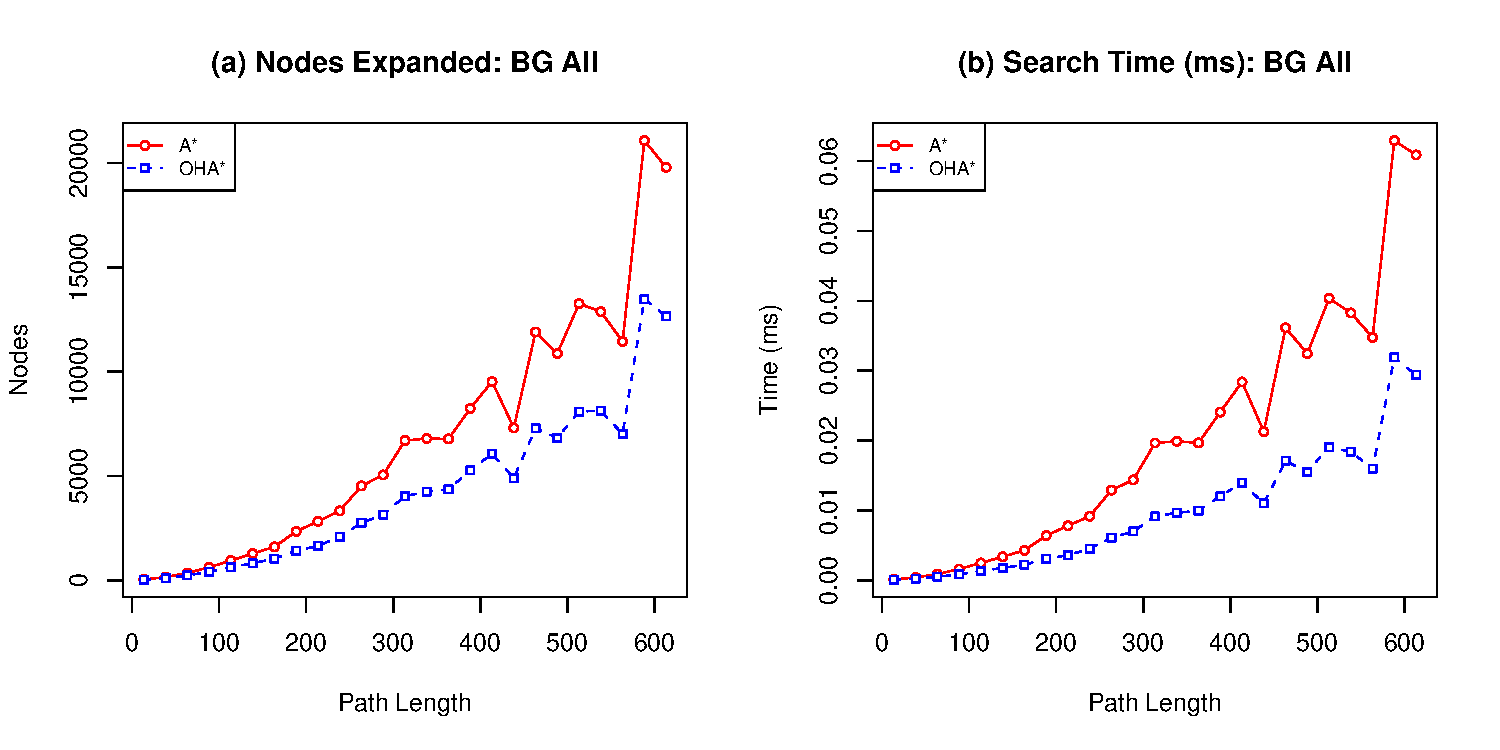
\includegraphics[scale=0.35, trim = 20mm 17mm 20mm 5mm]{diagrams/bg_effort.pdf}
	\end{center}
	\caption{Average number of nodes expanded across all maps in the Baldur's Gate set.}
	\label{fig-searcheffort}
	\vspace{-12pt}
\end{figure}
\par \indent
Figures \ref{fig-searcheffort}(a) and \ref{fig-searcheffort}(b)  show the average number of 
nodes expanded and generated. 
The trend is identical in both cases; OHA* expands and generates between 40-70\% fewer nodes than A*.
Problem instances with longer path lengths yield greater savings as on larger maps there is more 
opportunity for OHA* to prune nodes. 
Figure \ref{fig-searcheffort}(c) shows the corresponding search times for the problem instances. 
The same general trend may be observed; OHA* is between 1.7-2.1 times faster than A*.
We believe part of this speedup is attributable to the smaller open list OHA* needs to maintain.
We present data to support this hypothesis in Figure \ref{fig-searcheffort}(d) where we measure 
the maximum size of the open list. 
Notice that in the worst case OHA* is shown to maintain between 12-37\% fewer nodes where each
maintenance operation requires logarithmic time in the number of nodes.
\par
Finally, we turn our attention to Table \ref{table-csc2f} where we measure the 
performance of A* and OHA* on the six variants of CSC2F.
Our intention here is examine how the performance of OHA* degrades in scenarios with
high obstacle density.
\input csc2f_table
Observe that as the number of obstacles increases the number of nodes expanded by OHA*, and the
associated search time, both decrease. 
The drop in performance from R0 to R10 is quite significant; OHA*'s search times drop
from approximately 3 times faster than A* to just 1.36 times faster.
This advantage is further eroded as we go from R10 to R20 where OHA* is only 
1.23 times faster than A*.
Beyond this point the two algorithms can be considered equivalent;
OHA*'s map decomposition yields little advantage and the two expand and generate 
a very similar number of nodes.
